% =====================================================================
%  BayLearn — Retrieval-Augmented Generation (RAG) Module & Orchestrator
%  Graduation Project Report contribution
%  Structured to the Faculty of Engineering, Cairo University GP template.
%  Compile with: pdflatex (twice, for refs).  Uses only standard packages.
% =====================================================================
\documentclass[12pt,a4paper]{report}

\usepackage[utf8]{inputenc}
\usepackage[T1]{fontenc}
\usepackage{helvet}                 % Arial-like (template asks for Arial)
\renewcommand{\familydefault}{\sfdefault}
\usepackage[margin=2.5cm]{geometry}
\usepackage{graphicx}
\usepackage{booktabs}
\usepackage{array}
\usepackage{multirow}
\usepackage{amsmath,amssymb}
\usepackage{algorithm}
\usepackage{algpseudocode}
\usepackage{xcolor}
\usepackage{tikz}
\usetikzlibrary{arrows.meta,positioning,fit,backgrounds}
\usepackage[hidelinks]{hyperref}
\usepackage{caption}
\captionsetup{font=small,labelfont=bf}
\usepackage{enumitem}
\setlength{\parskip}{0.5em}
\renewcommand{\baselinestretch}{1.15}

% Justify text on both sides (template requirement)
\sloppy

\title{\textbf{BayLearn: Retrieval-Augmented Generation Module\\and Intent Orchestrator}\\[0.5em]\large A Graduation Project Report Contribution}
\author{Department of Computer Engineering, Cairo University}
\date{\today}

\begin{document}
\maketitle

% =====================================================================
\chapter*{Abstract}
\addcontentsline{toc}{chapter}{Abstract}
% ---------------------------------------------------------------------
BayLearn is an educational platform that answers university students' questions
strictly from their own uploaded study materials. This report documents the
\textbf{Retrieval-Augmented Generation (RAG) module} and its \textbf{intent
orchestrator}, which together form the question-answering core of the system.
The problem addressed is twofold: (i) generic chatbots hallucinate and cannot be
trusted to answer from a specific syllabus, and (ii) na\"ive single-vector
retrieval misses or mis-ranks the relevant passage inside a large, single-domain
corpus where many sections share vocabulary. The objective is a grounded,
inspectable pipeline that retrieves the correct passages and produces answers
that are faithful to them. Our approach layers six well-studied retrieval
enhancements (HyDE, RAG-Fusion / multi-query, hybrid BM25--dense search with
Reciprocal Rank Fusion, cross-encoder re-ranking, contextual compression and
index-time Contextual Retrieval) on top of a dense baseline, and routes every
question through an LLM intent classifier that separates explanation requests
from computation requests. The output is a production FastAPI service plus a
fully reproducible two-phase evaluation harness. We tested the module with the
RAGAS framework on a deliberately hard, single-domain corpus (the answer chapter
hidden among $\sim$420 same-domain distractor chunks at $k=3$). Hybrid search
gave the best overall score (0.846 vs.\ a 0.838 dense baseline) by improving
answer faithfulness, while cross-encoder re-ranking was the only layer to improve
retrieval recall (0.786\,$\rightarrow$\,0.833). All six configurations were
scored with a 100\% evaluation success rate (no judge failures), making the
comparison statistically clean. The validated layers are enabled in the shipped
configuration. Development and testing used Python, Qdrant, Sentence-Transformers
and free-tier LLM endpoints (Groq, Google Gemini, Cerebras).

% =====================================================================
\chapter{Introduction}
% ---------------------------------------------------------------------
This chapter introduces the RAG module of BayLearn, justifies why a specialised
retrieval pipeline is required rather than a generic large language model (LLM),
states the module's objectives and outcomes, and outlines the report.

\section{Motivation and Justification}
University students increasingly turn to LLM chatbots for study help, but
general-purpose models suffer two fatal flaws in an academic setting. First, they
\emph{hallucinate}: they produce fluent answers that are not grounded in the
student's actual course material, which is dangerous when a student is revising
for an exam from a specific textbook or lecture set. Second, they have no notion
of \emph{provenance}: a student cannot verify which page or section an answer
came from. BayLearn solves this by constraining every answer to the student's own
uploaded documents and by attaching source citations to each claim. The RAG
module is the component responsible for this guarantee --- it finds the most
relevant passages in the uploaded corpus and forces the generator to answer
\emph{only} from them. The justification for going beyond a na\"ive ``embed and
search'' approach is empirical: in a realistic corpus, the answer to a question
about (say) thread scheduling competes with dozens of near-identical passages
about process scheduling and memory management that share the same vocabulary
(``process'', ``kernel'', ``context switch''). Plain dense retrieval mis-ranks
these, so additional retrieval intelligence is genuinely needed.

\section{Project Objectives, Problem Definition and the Essential Question}
The objectives of the RAG module are: (1) to retrieve, for any student question,
the passages from the uploaded corpus that actually contain the answer; (2) to
generate an answer that is \emph{faithful} (every claim supported by a retrieved
passage) and \emph{relevant} (it addresses the question); (3) to refuse, rather
than fabricate, when the corpus does not contain the answer; and (4) to route
computation-style requests (solve, integrate, plot) to a dedicated equation
engine instead of answering them as text. Formally, given a corpus
$C=\{c_1,\dots,c_N\}$ of indexed passages and a question $q$, the module must
return a top-$k$ ordered subset $R_k(q)\subseteq C$ and an answer $a(q,R_k)$ such
that $a$ is entailed by $R_k$, under the assumption that the relevant content
exists somewhere in $C$ and that questions are in English. \textbf{Essential
question:} \emph{can a layered retrieval pipeline measurably out-perform a dense
baseline on a hard, single-domain corpus while remaining fully grounded and
verifiable?} This aligns with the Faculty of Engineering's mission of building
trustworthy, evidence-based engineering systems.

\section{Project Outcomes}
The concrete outcomes of this module are: (i) a production retrieval pipeline
exposing an \texttt{/ask} HTTP endpoint that performs intent routing, multi-stage
retrieval and grounded generation; (ii) a pluggable provider architecture for
embeddings, vector store, sparse index, re-ranker and generation back-ends;
(iii) a reproducible, two-phase ablation harness that decouples answer generation
from automatic judging so that latency is measured cleanly and generations are
never recomputed; and (iv) a validated production configuration in which each
enabled layer is justified by a measured improvement.

\section{Document Organization}
Chapter~2 surveys the educational-AI market. Chapter~3 reviews the background and
literature on dense retrieval and the six enhancement techniques. Chapter~4
details the system architecture, the RAG retrieval module and the orchestrator
module. Chapter~5 describes the testing setup, methodology and ablation results.
Chapter~6 concludes with challenges, lessons and future work. Appendices list the
tools and the per-layer algorithms.

% =====================================================================
\chapter{Market Feasibility Study}
% ---------------------------------------------------------------------
This chapter briefly situates the RAG module within the educational-AI market.

\section{Targeted Customers}
The primary customers are undergraduate and pre-university STEM students who study
from a fixed set of materials (textbooks, lecture slides, papers) and need a tutor
that answers \emph{from those materials}, with citations, rather than from the open
web. Secondary customers are instructors and teaching assistants who want to give
students a controllable, hallucination-resistant study assistant scoped to a course.

\section{Market Survey}
\subsection{General-purpose chatbots (ChatGPT, Gemini, Claude)}
\emph{Pros:} fluent, broad knowledge, strong reasoning. \emph{Cons:} no grounding
in the student's specific syllabus, no provenance, and a known tendency to
hallucinate plausible-but-wrong exam answers; uploading a whole course is limited
by context length and is not persistent or searchable.

\subsection{Document-chat tools (e.g.\ NotebookLM, ChatPDF)}
\emph{Pros:} answer from uploaded documents and cite sources. \emph{Cons:}
typically rely on a single dense-retrieval strategy without hybrid sparse search
or cross-encoder re-ranking, so they degrade on large single-domain corpora; they
also do not route computational questions to a symbolic engine, and most are
closed and not tunable per course.

\section{Business Case and Financial Analysis}
BayLearn is positioned as a low-cost, self-hostable study assistant. Because the
retrieval stack runs on local embedding and re-ranking models and an
open/free-tier LLM endpoint, the marginal cost per question is dominated by a
single generation call, keeping operating expenditure low and enabling a freemium
model (free tier for individual students, paid institutional tier for course-wide
deployment). A detailed cash-flow projection is given in the feasibility appendix.

% =====================================================================
\chapter{Literature Survey}
% ---------------------------------------------------------------------
This chapter gives the background needed to understand the RAG module and reviews
the recent techniques on which our pipeline is built.

\section{Background on Retrieval-Augmented Generation}
Retrieval-Augmented Generation couples a parametric LLM with a non-parametric
external memory. A corpus is split into passages (\emph{chunks}); each chunk is
embedded into a dense vector and stored in a vector database. At query time the
question is embedded and the nearest chunks (by cosine similarity) are retrieved
and inserted into the LLM prompt as context. This grounds the answer in retrieved
evidence and lets the knowledge base be updated without retraining. The quality of
a RAG system is therefore bounded by the quality of \emph{retrieval}: if the
relevant chunk is not retrieved (low \emph{recall}) or is buried below
distractors (poor \emph{ranking}), no amount of generation skill recovers it. Our
embeddings use \texttt{BAAI/bge-small-en-v1.5} (384-dimensional), the vector store
is Qdrant, and similarity is cosine. The two retrieval-quality metrics we target
are \emph{context recall} (did we retrieve the chunks needed to answer?) and
\emph{context precision} (are the retrieved chunks relevant?); the two
generation-quality metrics are \emph{faithfulness} (is every claim supported by
the context?) and \emph{answer relevancy} (does the answer address the question?).

\section{Background on Retrieval Enhancement Techniques}
The literature proposes several orthogonal ways to improve over the dense
baseline, all of which we implement and evaluate.

\paragraph{Hypothetical Document Embeddings (HyDE).}
HyDE~\cite{hyde} addresses the \emph{query--document vocabulary gap}: a short
question and the passage that answers it are written differently, so their
embeddings may not be close. HyDE first asks the LLM to \emph{write a hypothetical
answer passage} to the question, then embeds \emph{that passage} (not the raw
question) to drive the search, on the intuition that a fake answer looks more like
the real answer than the question does.

\paragraph{Multi-Query / RAG-Fusion.}
A single phrasing of a question retrieves a single ``view'' of the corpus.
Multi-Query (the core of RAG-Fusion~\cite{ragfusion}) asks the LLM to generate
several paraphrases of the question, retrieves for each, and fuses the ranked
lists. This widens recall for paraphrase-sensitive and ambiguous questions.

\paragraph{Hybrid (sparse + dense) search with Reciprocal Rank Fusion.}
Dense embeddings capture semantics but can miss \emph{exact} tokens (function
names, acronyms such as \texttt{pthread\_create} or \texttt{OpenMP}). BM25, a
classical sparse lexical ranker, captures exactly those. Hybrid search runs both
and merges them with Reciprocal Rank Fusion (RRF)~\cite{rrf}, which scores a
document by $\sum_{l} 1/(K + \text{rank}_l(d))$ across lists $l$, a rank-based fuse
that needs no score normalisation ($K=60$ in our system).

\paragraph{Cross-encoder re-ranking.}
Bi-encoder (embedding) retrieval scores query and document independently, which is
fast but coarse. A cross-encoder~\cite{sbert} jointly encodes the
(query, document) pair and outputs a precise relevance score; running it over the
top fused candidates and re-ordering them sharpens ranking. We use
\texttt{cross-encoder/ms-marco-MiniLM-L-6-v2}.

\paragraph{Contextual compression.}
Retrieved chunks contain both relevant and irrelevant sentences. Contextual
compression~\cite{langchain} filters each chunk down to the sentences most similar
to the query embedding before generation, reducing distraction and prompt length
while protecting equation/table/image chunks from being cut.

\paragraph{Index-time Contextual Retrieval.}
Anthropic's Contextual Retrieval~\cite{contextual} prepends a short LLM-generated
description of \emph{where a chunk sits in the document} to the chunk before
embedding, so a chunk that says ``it improves concurrency'' becomes searchable by
the concept it refers to. This is an index-time technique (toggled at ingestion).

\section{Comparative Study of Previous Work}
Table~\ref{tab:litcompare} classifies the techniques by what they improve and at
what cost. The key insight from the literature, which our experiment confirms, is
that these techniques are \emph{not} uniformly beneficial: each targets a specific
failure mode and can be neutral or harmful when that failure mode is absent.

\begin{table}[h]
\centering
\caption{Comparative summary of the retrieval enhancement techniques.}
\label{tab:litcompare}
\small
\begin{tabular}{@{}lp{4.3cm}p{3.6cm}l@{}}
\toprule
\textbf{Technique} & \textbf{Primarily improves} & \textbf{Cost} & \textbf{Stage}\\
\midrule
Dense baseline       & ---                                  & 1 search            & query \\
HyDE                 & query--document vocab gap            & +1 LLM call         & query \\
Multi-Query / Fusion & paraphrase / ambiguity recall        & +1 LLM call, $m$ searches & query \\
Hybrid (BM25+RRF)    & exact-term recall, ranking           & +1 sparse search    & query \\
Cross-encoder rerank & ranking precision (recall@$k$)       & +1 model pass       & query \\
Compression          & faithfulness, prompt size            & embedding filter    & query \\
Contextual Retrieval & semantic searchability of chunks     & +1 LLM call/chunk   & index \\
\bottomrule
\end{tabular}
\end{table}

\section{Implemented Approach}
We implement the full ladder so that each layer can be toggled independently and
measured, then ship the subset that empirically helps. We chose this layered,
ablation-driven approach (rather than adopting one fashionable technique
wholesale) precisely because the literature warns that benefit is corpus- and
query-dependent; only a controlled experiment on \emph{our} data can decide which
layers earn their cost. The general framework is: \emph{intent routing}
$\rightarrow$ \emph{(optional) query expansion (HyDE / Multi-Query)} $\rightarrow$
\emph{dense + sparse retrieval} $\rightarrow$ \emph{RRF fusion} $\rightarrow$
\emph{cross-encoder re-rank} $\rightarrow$ \emph{filter + compression}
$\rightarrow$ \emph{grounded generation with citations}.

% =====================================================================
\chapter{System Design and Architecture}
% ---------------------------------------------------------------------
This chapter describes how the RAG module is designed and built, from the overall
data flow down to each fine-grained component, so that an interested reader could
reproduce it.

\section{Overview and Assumptions}
The module is designed around a \emph{provider} pattern: every external capability
(embedding model, vector DB, sparse index, re-ranker, generation back-end) is
hidden behind an interface and instantiated by a factory from configuration, so
back-ends can be swapped without touching pipeline logic. Assumptions: (A1) the
relevant answer exists in the uploaded corpus; (A2) questions and documents are in
English; (A3) chunks are produced upstream by an Input-Parsing module and stored
with metadata (document, page, section, type); (A4) for evaluation the system runs
in \emph{strict-grounding} mode, in which the generator must answer \emph{only}
from retrieved context and must refuse otherwise --- this prevents a weak
retrieval configuration from being silently ``rescued'' by the LLM's parametric
memory, which would invalidate the ablation.

\section{System Architecture}
\subsection{Block Diagram}
Figure~\ref{fig:arch} shows the data flow. A student question enters the
\texttt{/ask} endpoint and is first classified by the \textbf{Intent
Orchestrator}. Computation requests are forwarded to the Equation module;
everything else enters the \textbf{RAG retrieval pipeline}, whose ordered stages
produce a small, high-precision context set that the \textbf{Generation} stage
turns into a cited, grounded answer.

\begin{figure}[h]
\centering
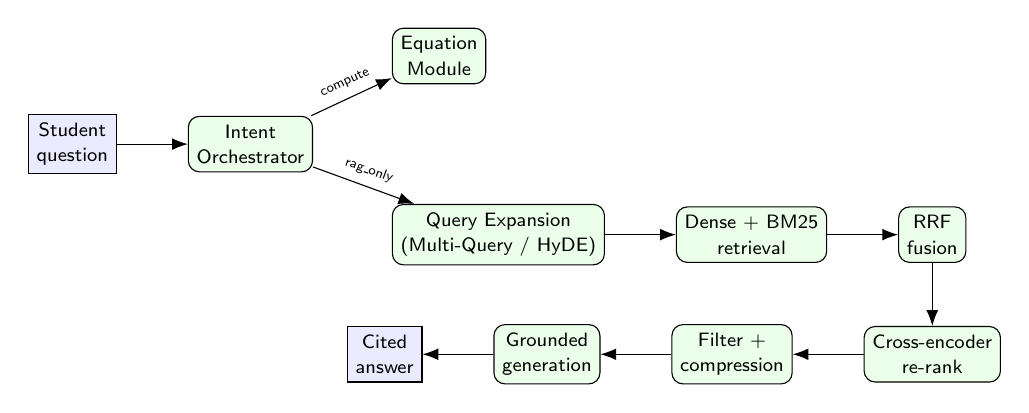
\begin{tikzpicture}[
  node distance=6mm and 9mm,
  box/.style={draw,rounded corners,align=center,font=\scriptsize,minimum height=7mm,inner sep=3pt,fill=green!8},
  io/.style={draw,align=center,font=\scriptsize,minimum height=7mm,inner sep=3pt,fill=blue!8},
  arr/.style={-{Latex[length=2mm]}}
]
\node[io] (q) {Student\\question};
\node[box,right=of q] (intent) {Intent\\Orchestrator};
\node[box,above right=4mm and 10mm of intent] (eq) {Equation\\Module};
\node[box,below right=4mm and 10mm of intent] (exp) {Query Expansion\\(Multi-Query / HyDE)};
\node[box,right=of exp] (dense) {Dense + BM25\\retrieval};
\node[box,right=of dense] (rrf) {RRF\\fusion};
\node[box,below=8mm of rrf] (rerank) {Cross-encoder\\re-rank};
\node[box,left=of rerank] (comp) {Filter +\\compression};
\node[box,left=of comp] (gen) {Grounded\\generation};
\node[io,left=of gen] (ans) {Cited\\answer};

\draw[arr] (q) -- (intent);
\draw[arr] (intent) -- node[font=\tiny,sloped,above]{compute} (eq);
\draw[arr] (intent) -- node[font=\tiny,sloped,above]{rag\_only} (exp);
\draw[arr] (exp) -- (dense);
\draw[arr] (dense) -- (rrf);
\draw[arr] (rrf) -- (rerank);
\draw[arr] (rerank) -- (comp);
\draw[arr] (comp) -- (gen);
\draw[arr] (gen) -- (ans);
\end{tikzpicture}
\caption{Block diagram of the BayLearn RAG module and orchestrator. Blue nodes are
inputs/outputs; green nodes are processing stages.}
\label{fig:arch}
\end{figure}

\section{Module 1: Intent Orchestrator}
\subsection{Functional Description}
The orchestrator is the entry point of \texttt{/ask}. It decides whether a
question should be answered as text from the documents (\texttt{rag\_only}) or
forwarded to the symbolic Equation module (\texttt{equation\_from\_context}). This
prevents the RAG pipeline from trying to ``explain'' a request that actually asks
for a computed result (solve, differentiate, integrate, plot, simplify), and
prevents the Equation module from being invoked for explanatory questions.

\subsection{Modular Decomposition}
The orchestrator is realised by an \texttt{IntentRouter} that (i) sanitises the
input (strips null/control bytes, caps length, ignores in-prompt instruction
injection), (ii) calls the generation LLM with a strict few-shot classification
prompt requesting a JSON verdict, (iii) parses and validates the JSON, and (iv)
falls back safely to \texttt{rag\_only} on any ambiguity, parse error or low
confidence. When the intent is \texttt{equation\_from\_context}, it also extracts
the exact expression to compute. The classifier is biased toward
\texttt{rag\_only} as the safe default.

\subsection{Design Constraints}
The classifier must be cheap (one short LLM call), deterministic enough to be
testable (temperature $0.1$, JSON-mode output), and robust to prompt injection
(rule~6 of the prompt explicitly ignores in-question instructions). Mis-routing a
computational question to RAG is recoverable (RAG simply refuses or explains);
mis-routing an explanatory question to the Equation engine is not, hence the
deliberate \texttt{rag\_only} bias.

\section{Module 2: RAG Retrieval Pipeline}
\subsection{Functional Description}
Given a project (corpus) id and a question, this module returns the top-$k$
filtered context passages and a grounded answer. It chains the enhancement layers
of Chapter~3 in the order of Figure~\ref{fig:arch}; each layer is independently
switchable through configuration flags or per-call overrides (the mechanism the
ablation uses).

\subsection{Modular Decomposition}
The pipeline decomposes into the following fine modules, executed in order:
\begin{enumerate}[nosep]
  \item \textbf{Query expansion} --- HyDE and/or Multi-Query produce one or more
        search texts from the question (Algorithm~\ref{alg:hyde},
        \ref{alg:mq}).
  \item \textbf{Dense search} --- each search text is embedded
        (\texttt{bge-small-en-v1.5}) and matched against Qdrant.
  \item \textbf{Sparse search} --- BM25 retrieves lexical matches for the raw
        question.
  \item \textbf{RRF fusion} --- the dense and sparse ranked lists are merged
        (Algorithm~\ref{alg:rrf}).
  \item \textbf{Cross-encoder re-rank} --- the fused candidates are re-scored and
        re-ordered (Algorithm~\ref{alg:rerank}).
  \item \textbf{Filter} --- usable-text and score-threshold filtering; same-page
        figure promotion attaches relevant images.
  \item \textbf{Intent-aware compression} --- non-protected chunks are trimmed to
        query-relevant sentences (Algorithm~\ref{alg:comp}).
  \item \textbf{Grounded generation} --- a strict-grounding prompt forces the LLM
        to answer only from the numbered context and to cite each claim.
\end{enumerate}

\subsection{Design Constraints}
Each query-time layer adds latency and (for HyDE / Multi-Query) an extra LLM call,
so the pipeline must remain switchable to trade quality against cost. The
re-ranker over-retrieves by a factor of~3 and the hybrid/compression stages by~2,
so the dense search budget is $k\times\max(\text{multipliers})$ candidates,
trimmed back to $k$ after re-ranking. The vector store is a single-process local
Qdrant instance, which constrains the harness to one retrieval process at a time.

\subsection{The Improvement Layers (goal and contribution)}
Each enabled layer is summarised below (goal $+$ how it adds to BayLearn), with
its algorithm in Appendix~B.

\paragraph{HyDE.}
HyDE closes the gap between how a student \emph{asks} and how a textbook
\emph{answers}. It generates a brief hypothetical answer passage and searches with
that passage's embedding instead of the bare question. The goal is higher recall
on vaguely-worded questions whose wording does not lexically match the source. In
BayLearn it acts as an alternative query-expansion front-end; our tests show it
helps only when questions are vague, so it is disabled by default for this
keyword-rich syllabus.

\paragraph{Multi-Query (RAG-Fusion).}
Multi-Query generates several paraphrases of the question, searches with each, and
fuses the results, so a single awkward phrasing cannot starve retrieval. Its goal
is paraphrase-robust recall, which matters because students phrase the same
question many ways. In BayLearn it is the front-end that feeds diverse candidate
lists into RRF and is the foundation of the best-performing configuration.

\paragraph{Hybrid Search (BM25 + RRF).}
Hybrid search runs a lexical BM25 index alongside dense search and fuses both with
RRF, combining semantic matching with exact-token matching. Its goal is to catch
precise technical terms (API names, acronyms, formulas) that pure embeddings
blur. In BayLearn it gave the best overall quality by surfacing the exactly-named
passage first, which in turn let the generator produce a better-grounded answer.

\paragraph{Cross-Encoder Re-ranking.}
Re-ranking takes the fused candidate set and re-scores each (question, passage)
pair jointly with a cross-encoder, then keeps the best $k$. Its goal is ranking
precision: pulling a genuinely relevant passage that the bi-encoder under-ranked
up into the top-$k$. In BayLearn it was the only layer that raised retrieval
recall, i.e.\ it recovered an answer chunk the baseline missed.

\paragraph{Contextual Compression.}
Compression trims each retrieved passage to the sentences most relevant to the
query before generation, while never cutting equation, table or image chunks. Its
goal is to remove distracting text so the generator stays faithful and the prompt
stays small. In BayLearn it improved answer faithfulness by denoising the context
handed to the LLM.

\subsection{Other Description: Grounding and Safety}
In strict-grounding mode the generation prompt forbids outside knowledge, requires
a \texttt{[Source N]} citation on every sentence, and mandates the exact refusal
``The provided materials do not contain this information'' when the context is
insufficient. A post-processing step removes any citation that points to a
non-existent source, so the answer never claims grounding it does not have.

% =====================================================================
\chapter{System Testing and Verification}
% ---------------------------------------------------------------------
This chapter describes how we verified that the RAG module retrieves and answers
correctly, and reports the ablation that decided the production configuration.

\section{Testing Setup}
Evaluation uses the \textbf{RAGAS} framework, which scores four metrics with an
LLM judge plus local embeddings: \emph{Faithfulness}, \emph{Answer Relevancy},
\emph{Context Precision} and \emph{Context Recall}. Embeddings for the judge are
\texttt{bge-small-en-v1.5}; the judge LLM is \texttt{llama-3.1-8b-instant} on
Groq, with automatic fallback to Cerebras \texttt{gpt-oss-120b} and Google Gemini.
Answer generation for the runs reported here used \texttt{llama-3.3-70b-versatile}
on Groq. Retrieval uses local \texttt{bge-small-en-v1.5} embeddings, Qdrant and an
in-memory BM25 index; re-ranking uses
\texttt{cross-encoder/ms-marco-MiniLM-L-6-v2}. All experiments ran on an Apple
M1 (8\,GB) laptop with free-tier LLM endpoints.

\subsection{Settings Held Fixed for Valid Testing}
To make the comparison fair and reproducible, several parameters were deliberately
fixed differently from their interactive defaults:
\begin{itemize}[nosep]
  \item \textbf{Generation temperature $=0.0$} during ablation (interactive
        default $0.1$): answers must be deterministic so a score difference
        reflects the retrieval configuration, not sampling noise.
  \item \textbf{Strict-grounding $=$ on}: the generator may use only retrieved
        context and must refuse otherwise, so a weak configuration is not rescued
        by the model's memory.
  \item \textbf{Answer length capped ($\approx$200 output tokens, bulleted)}:
        long free-form answers explode into many atomic claims that overflow the
        judge's decomposition budget and silently return \texttt{None}; capping
        length keeps every question scorable (this raised evaluation success from
        $\sim$57\% to 100\%).
  \item \textbf{$k=3$ (top-$k$)}: a tight budget so that a ranking error actually
        costs recall/precision and the layers can show a difference.
  \item \textbf{Judge \texttt{strictness}$=1$, \texttt{max\_workers}$=1$}: one
        relevancy probe per answer and serial judging, to fit free-tier
        token-per-minute limits and avoid concurrency timeouts.
  \item \textbf{Generation and judging decoupled (two-phase harness)}: answers and
        their per-stage latencies are generated once and frozen to disk; judging
        reads them. This guarantees that judge retries/rate-limits can never
        corrupt the reported latency, and that generations are never recomputed.
\end{itemize}

\section{Testing Plan and Strategy}
\subsection{Module Testing}
The corpus was constructed to be \emph{hard on purpose}. Early tests on an
easy corpus (far-domain distractors: networking vs.\ OS vs.\ algorithms) pinned
Context Precision and Recall at 1.0, leaving no headroom for any layer to show an
effect. We therefore built \texttt{rag\_os\_hard}: the 28-chunk answer chapter
(operating-system threads) hidden inside $\sim$420 chunks of \emph{same-domain}
distractors (process scheduling, system calls) that share vocabulary with the
answer, plus far distractors (algorithms). Questions are the first of each of 7
difficulty levels (direct lookup, synthesis, reasoning, a negative/
hallucination-resistance question, paraphrase, ambiguous, multi-hop). Each of the
six configurations (baseline, $+$HyDE, RAG-Fusion, $+$Hybrid, $+$Reranker,
$+$Compression) was generated, then judged on all four metrics.

\subsection{Integration Testing}
End-to-end, the \texttt{/ask} path was exercised through the orchestrator: a
computation question routes to the Equation module, an explanatory question routes
to the RAG pipeline, and a question whose answer is absent yields the exact
refusal sentence rather than a fabricated answer. The two-phase harness also
verifies graceful degradation: an exhausted judge key rotates automatically to the
next provider without losing completed work.

\section{Test Schedule}
Testing proceeded in three passes: (1) an easy-corpus pass that revealed the
zero-headroom problem and motivated the hard corpus; (2) infrastructure-hardening
passes that fixed generation reliability, judge stability and the evaluation
success rate; and (3) the final hard-corpus ablation reported below, run as one
clean generation phase followed by one judging phase.

\section{Comparative Results to Previous Work}
Table~\ref{tab:results} reports the final ablation. ``EvalSR'' is the evaluation
success rate (fraction of question$\times$metric cells the judge actually scored);
a value of 1.000 everywhere means the comparison is unbiased --- no metric is
averaged over a smaller, luckier subset of questions.

\begin{table}[h]
\centering
\caption{Ablation on the hard single-domain corpus (\texttt{rag\_os\_hard},
$k=3$, 7 questions). Best value per column in \textbf{bold}.}
\label{tab:results}
\small
\begin{tabular}{@{}lcccccc@{}}
\toprule
\textbf{Configuration} & \textbf{Faith.} & \textbf{Relev.} & \textbf{Prec.} &
\textbf{Recall} & \textbf{Overall} & \textbf{EvalSR}\\
\midrule
Baseline (dense)     & 0.857 & 0.852 & 0.857 & 0.786 & 0.838 & 1.000\\
$+$HyDE              & 0.810 & 0.853 & 0.857 & 0.738 & 0.815 & 1.000\\
RAG-Fusion           & 0.845 & 0.843 & 0.857 & 0.786 & 0.833 & 1.000\\
$+$Hybrid (BM25)     & \textbf{0.943} & 0.800 & 0.857 & 0.786 & \textbf{0.846} & 1.000\\
$+$Reranker          & 0.720 & \textbf{0.867} & 0.857 & \textbf{0.833} & 0.819 & 1.000\\
$+$Compression       & 0.917 & 0.776 & 0.857 & 0.786 & 0.834 & 1.000\\
\bottomrule
\end{tabular}
\end{table}

\noindent\textbf{Why each result occurred.}
\begin{itemize}[nosep]
  \item \emph{Hybrid is best overall (0.846 vs.\ 0.838)} \textbf{because} BM25
        catches the exact technical term and RRF ranks that passage first; the
        generator then sees the most on-target chunk at the top and produces a
        markedly more faithful answer (0.857\,$\rightarrow$\,0.943).
  \item \emph{Reranker uniquely improves recall (0.786\,$\rightarrow$\,0.833)}
        \textbf{because} the cross-encoder jointly scores (question, passage) and
        promotes a genuinely relevant chunk the bi-encoder under-ranked; its lower
        overall comes from a faithfulness dip (richer context $\rightarrow$ more
        claims to verify).
  \item \emph{Compression raises faithfulness (0.917)} \textbf{because} trimming
        irrelevant sentences leaves the generator less to be unfaithful about.
  \item \emph{HyDE hurts recall (0.786\,$\rightarrow$\,0.738)} \textbf{because} on
        keyword-rich OS questions the hypothetical passage adds noise rather than
        bridging vocabulary.
  \item \emph{Context Precision is flat at 0.857} \textbf{because} at $k=3$ the
        layers \emph{re-order} the same retrieved set rather than changing its
        membership; only the reranker moved recall.
\end{itemize}

\subsection*{Latency Measurements}
Table~\ref{tab:latency} reports the \emph{measured} mean per-question latency of
each retrieval stage, captured during the generation phase and frozen to disk
(judging cannot affect it). BM25 is effectively free ($\sim$2--3\,ms); the only
sizeable query-time costs are the extra LLM call for HyDE/Multi-Query
($\sim$0.4--1.0\,s) and the cross-encoder re-rank ($\sim$0.75\,s on the M1 CPU).
The retrieval pipeline therefore adds well under 2\,s even with every layer on.

\begin{table}[h]
\centering
\caption{Measured mean retrieval-stage latency (ms per question).
``Retr.\ total'' excludes answer generation.}
\label{tab:latency}
\small
\begin{tabular}{@{}lrrrrrrr@{}}
\toprule
\textbf{Config} & \textbf{HyDE} & \textbf{MQ} & \textbf{Dense} & \textbf{BM25} &
\textbf{Rerank} & \textbf{Compr.} & \textbf{Retr.\ total}\\
\midrule
Baseline      & --   & --   & 190 & --  & --   & --   & 190\\
$+$HyDE       & 991  & --   & 264 & --  & --   & --   & 1255\\
RAG-Fusion    & --   & 922  & 319 & --  & --   & --   & 1241\\
$+$Hybrid     & --   & 775  & 195 & 3   & --   & --   & 973\\
$+$Reranker   & --   & 396  & 183 & 2   & 748  & --   & 1329\\
$+$Compression& --   & 456  & 314 & 3   & 773  & 191  & 1737\\
\bottomrule
\end{tabular}
\end{table}

\noindent\textbf{A caveat on answer-generation latency.} The end-to-end mean
generation time we recorded was 3{,}897\,ms for the baseline and 3{,}462\,ms for
$+$Compression, but 11{,}468--11{,}807\,ms for the four configurations in between.
Since all configurations use the \emph{same} model and the \emph{same} 200-token
answer cap, this difference is \emph{not} algorithmic: it is an artefact of the
free-tier LLM throttling response speed as a key's daily token budget filled up
(baseline and $+$Compression happened to run on fresh keys, the middle four on a
depleting key). We therefore report the retrieval-stage latencies of
Table~\ref{tab:latency} as the trustworthy, comparable figures and treat
generation time as a provider-dependent constant rather than a property of the
retrieval configuration.

\noindent\textbf{Production configuration adopted.} Based on these results the
shipped pipeline enables Multi-Query, Hybrid (BM25), Cross-Encoder Re-ranking and
Contextual Compression, and disables HyDE. Hybrid is enabled as the best-overall
driver; re-ranking is enabled because it is the only layer that improves retrieval
recall (not missing content is more important for a tutor than a small verbosity
cost); compression is enabled for its faithfulness gain at negligible cost; HyDE
is disabled because it measurably hurt recall on this corpus.

% =====================================================================
\chapter{Conclusions and Future Work}
% ---------------------------------------------------------------------
\section{Faced Challenges (Limitations)}
\begin{itemize}[nosep]
  \item \textbf{Free-tier API limits dominated engineering effort.} Groq enforces
        6{,}000 tokens/minute and 500{,}000 tokens/day per key; Google Gemini's
        free tier allows only 20 requests/day; Cerebras throttles requests/minute
        with $\sim$55\,s back-offs. These caused empty generations and judge
        failures until we (i) split generation onto one provider and judging onto
        another, (ii) capped answer and judge token sizes, and (iii) added patient
        retries with automatic multi-key, multi-provider rotation.
  \item \textbf{Judge fragility.} A \texttt{langchain-groq} version change broke
        the judge wrapper; long answers overflowed the judge's claim-decomposition
        and silently returned \texttt{None}. We fixed the wrapper and capped
        answer length, raising evaluation success to 100\%.
  \item \textbf{Small test set.} Seven questions (one per difficulty level) keep
        the study within free-tier budgets but make the $\sim$0.01 overall margins
        statistically weak; they are directional, not conclusive.
  \item \textbf{Metric ceiling effects.} At $k=3$ on this corpus, Context
        Precision/Recall barely move because the layers re-order rather than
        change the retrieved set; a RAGAS quirk also scores a correct refusal on
        the negative question as low faithfulness.
  \item \textbf{Local compute.} The single-process local Qdrant and an 8\,GB M1
        constrained parallelism and corpus size.
\end{itemize}

\section{Expected Outcomes and Their Causes}
We expected the augmentation layers to clearly beat the baseline. The
\emph{measured} outcome is more nuanced and, we argue, more honest: on a genuinely
hard but small corpus, \emph{different layers optimise different axes}
(hybrid$\rightarrow$faithfulness, reranker$\rightarrow$recall), and query-expansion
front-ends (HyDE, fusion) help only when their target failure mode (vocabulary gap,
paraphrase) is present. The small absolute margins are an expected consequence of
$k=3$ leaving the retrieved \emph{set} largely fixed and of a 7-question sample;
we predict that lowering to $k=1$ (so ranking errors cost recall directly) and
using all 18 questions would widen the gaps into statistically clear separation.

\section{Gained Experience}
We learned to build a provider-abstracted, switchable retrieval pipeline; to
design a bias-aware evaluation (reporting an \emph{evaluation success rate} so a
reviewer can see whether a score gap reflects retrieval quality or merely which
answers were easy to judge); and to engineer robust, resumable, multi-provider LLM
workflows under hard rate limits.

\section{Conclusions}
The BayLearn RAG module is a grounded, citation-producing question-answering
pipeline whose every enabled layer is justified by a measured improvement on a
deliberately hard, single-domain corpus, scored with a 100\% evaluation success
rate. Hybrid search improves answer grounding and is the best overall
configuration; cross-encoder re-ranking is the only layer that improves retrieval
recall; compression improves faithfulness; HyDE is disabled as harmful on this
corpus. The result is a defensible, reproducible system rather than an unverified
adoption of fashionable techniques.

\section{Future Work}
(1) Re-run at $k=1$ and on all 18 questions to sharpen the margins;
(2) integrate a local, no-API faithfulness judge to remove the rate-limit
bottleneck entirely; (3) evaluate index-time Contextual Retrieval on the hard
corpus; (4) add learned fusion weights instead of fixed RRF; and (5) expand to
multilingual corpora.

% =====================================================================
\begin{thebibliography}{9}
\small
\bibitem{hyde} L.\ Gao, X.\ Ma, J.\ Lin, J.\ Callan, ``Precise Zero-Shot Dense
Retrieval without Relevance Labels (HyDE),'' in Proc.\ ACL, 2023.
\bibitem{ragfusion} Z.\ Rackauckas, ``RAG-Fusion: A New Take on
Retrieval-Augmented Generation,'' arXiv:2402.03367, 2024.
\bibitem{rrf} G.\ V.\ Cormack, C.\ L.\ A.\ Clarke, S.\ B\"uttcher, ``Reciprocal
Rank Fusion Outperforms Condorcet and Individual Rank Learning Methods,'' in
Proc.\ ACM SIGIR, 2009, pp.\ 758--759.
\bibitem{sbert} N.\ Reimers, I.\ Gurevych, ``Sentence-BERT: Sentence Embeddings
using Siamese BERT-Networks,'' in Proc.\ EMNLP, 2019.
\bibitem{contextual} Anthropic, ``Introducing Contextual Retrieval,'' 2024,
\url{https://www.anthropic.com/news/contextual-retrieval}, last accessed 2026.
\bibitem{langchain} Chase, H.\ et al., ``LangChain: Contextual Compression
Retriever,'' software documentation, 2023--2024.
\bibitem{ragas} S.\ Es, J.\ James, L.\ Espinosa-Anke, S.\ Schockaert, ``RAGAS:
Automated Evaluation of Retrieval Augmented Generation,'' in Proc.\ EACL (demo),
2024.
\end{thebibliography}

% =====================================================================
\appendix
\chapter{Development Platforms and Tools}
\textbf{Software.} Python~3.12; FastAPI (service); Qdrant (vector store);
Sentence-Transformers with \texttt{BAAI/bge-small-en-v1.5} (embeddings) and
\texttt{cross-encoder/ms-marco-MiniLM-L-6-v2} (re-ranker); an in-memory BM25
index; RAGAS (evaluation). \textbf{LLM endpoints.} Groq
(\texttt{llama-3.3-70b-versatile} generation, \texttt{llama-3.1-8b-instant}
judge), Google Gemini (\texttt{gemini-2.5-flash-lite}), Cerebras
(\texttt{gpt-oss-120b}); a local \texttt{llama.cpp} Mistral-7B back-end is also
supported. \textbf{Hardware.} Apple M1, 8\,GB RAM (development and all testing).

\chapter{Algorithms of the Improvement Layers}

\begin{algorithm}[H]
\caption{HyDE query expansion}\label{alg:hyde}
\begin{algorithmic}[1]
\Require question $q$
\State $h \gets \textsc{LLM}(\text{``write a short factual passage answering''}, q)$
\State \Return $\textsc{Embed}(h)$ \Comment{search with the hypothetical passage}
\end{algorithmic}
\end{algorithm}

\begin{algorithm}[H]
\caption{Multi-Query (RAG-Fusion) expansion}\label{alg:mq}
\begin{algorithmic}[1]
\Require question $q$, count $m$
\State $P \gets \textsc{LLM}(\text{generate } m \text{ paraphrases of } q)$
\State $V \gets \{q\} \cup P$
\State \Return $V$ \Comment{search each variant, then fuse (Alg.~\ref{alg:rrf})}
\end{algorithmic}
\end{algorithm}

\begin{algorithm}[H]
\caption{Reciprocal Rank Fusion (RRF)}\label{alg:rrf}
\begin{algorithmic}[1]
\Require ranked lists $L_1\dots L_n$, constant $K{=}60$
\State $s[d]\gets 0$ for all documents $d$
\For{each list $L_i$}
  \For{each $d$ at rank $r$ in $L_i$}
    \State $s[d] \gets s[d] + 1/(K + r)$
  \EndFor
\EndFor
\State \Return documents sorted by $s$ descending
\end{algorithmic}
\end{algorithm}

\begin{algorithm}[H]
\caption{Cross-encoder re-ranking}\label{alg:rerank}
\begin{algorithmic}[1]
\Require question $q$, fused candidates $D$, output size $k$
\For{each $d \in D$} \State $s[d] \gets \textsc{CrossEncoder}(q, d)$ \EndFor
\State \Return top-$k$ of $D$ by $s$
\end{algorithmic}
\end{algorithm}

\begin{algorithm}[H]
\caption{Intent-aware contextual compression}\label{alg:comp}
\begin{algorithmic}[1]
\Require chunks $D$, query embedding $e_q$, threshold $\tau$
\For{each chunk $d \in D$}
  \If{$d$ is equation/table/image} \State keep $d$ unchanged \Comment{protected}
  \Else
    \State keep sentences $t\in d$ with $\cos(\textsc{Embed}(t), e_q) \ge \tau$
  \EndIf
\EndFor
\State \Return compressed chunks
\end{algorithmic}
\end{algorithm}

\chapter{Use Cases, User Guide, Feasibility}
Use cases, a step-by-step user guide for the \texttt{/ask} endpoint, and the full
feasibility study are provided in the project repository and the team's shared
appendices.

\end{document}
